\begin{figure}[h]
    \centering
    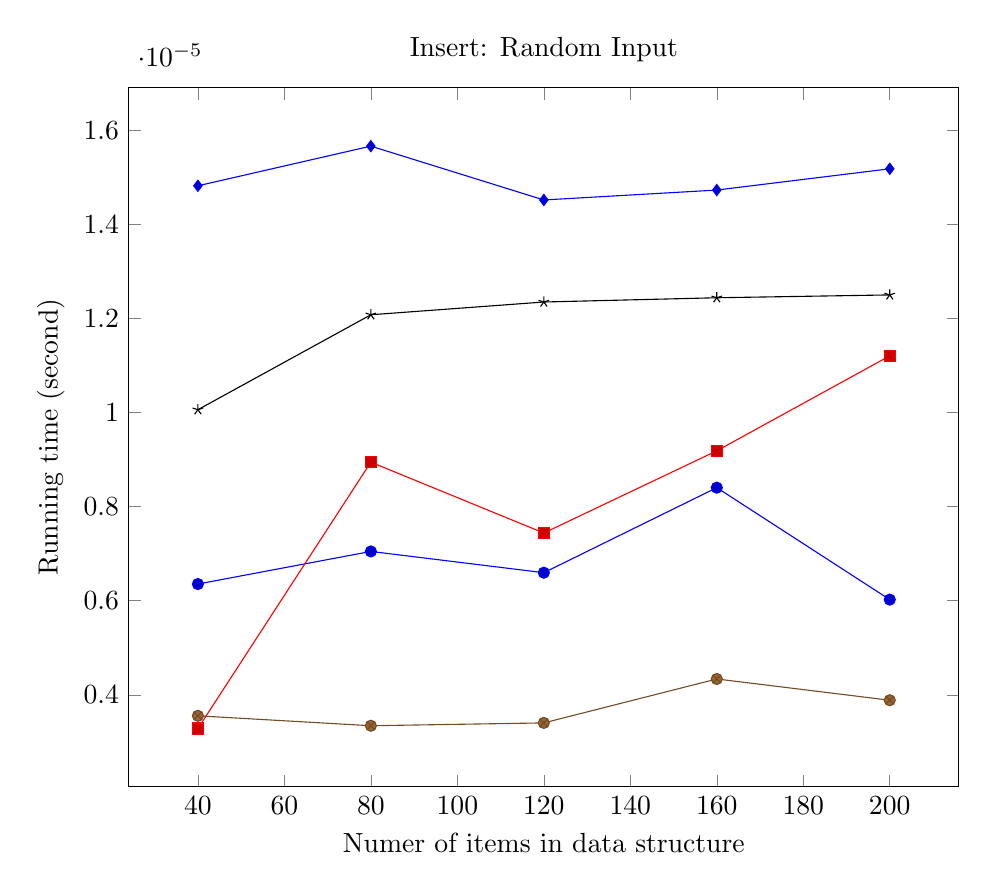
\begin{tikzpicture}
        \begin{axis}[
            xlabel={Numer of items in data structure},
            ylabel={Running time (second)},
            title={Insert: Random Input},
            width=\textwidth
        ]
		\addplot coordinates {
			(200, 6.023506734820217e-06)
			(160, 8.402791895179007e-06)
			(120, 6.59573987462636e-06)
			(80, 7.047502879942158e-06)
			(40, 6.354799605645667e-06)
		};
		\addplot coordinates {
			(200, 1.120372252714219e-05)
			(160, 9.185847770964984e-06)
			(120, 7.439030817835146e-06)
			(80, 8.944907501629017e-06)
			(40, 3.2828111706351136e-06)
		};
		\addplot coordinates {
			(200, 3.885161844152662e-06)
			(160, 4.336924849113189e-06)
			(120, 3.4032813051254608e-06)
			(80, 3.343046238057923e-06)
			(40, 3.5538689736824836e-06)
		};
		\addplot coordinates {
			(200, 1.2498776475311502e-05)
			(160, 1.2438541407888692e-05)
			(120, 1.234818880675448e-05)
			(80, 1.2077131003707109e-05)
			(40, 1.0059256247529902e-05)
		};
		\addplot coordinates {
			(200, 1.5179236972429067e-05)
			(160, 1.472747396746854e-05)
			(120, 1.4516651231133437e-05)
			(80, 1.5661117511100996e-05)
			(40, 1.4817826568247482e-05)
		};
        \legend{}
        \end{axis}
    \end{tikzpicture}
    \caption{Average of 0 operations, benchmarked every 0, starting at 0.}
\end{figure}